\section{Grafer og grafalgoritmer}
Ofte har vi ikke bare ett sett med elementer som skal behandles men også forbindelser mellom disse. Dette kan representeres ved hjelp av en graf.
\\\\
En graf, $G = (V,E)$, består av noder (V for \textit{vertices}) og kanter (E for \textit{edges}). Begge deler kan inneholde informasjon. For eksempel kan nodene være hus og kantene være veier mellom husene. Veiene kan ha ulik lengde eller andre egenskaper som gjør at hvilken vei vi velger ikke er avhengig av hvor mange hus vi må innom. Vi sier at kantene har forskjellige kostnader. Dessuten kan veiene være enveiskjørte.

\begin{itemize}
    \item \textbf{Naboer:} To noder er \textit{naboer} dersom det går en kant mellom dem. Nabonoder sies å være \textit{adjacent}.
    \item \textbf{Rettet:} Vi har en \textit{rettet graf} (\textit{firected path}) dersom kantene har retning og kun kan brukes den ene veien (piler).
    \item \textbf{Urettet:} En graf er \textit{urettet} (\textit{undirected}) dersom kantene ikke har noen spesiell retning og kan brukes begge veier.
    \item \textbf{Sykel:} Vi har en \textit{sykel} i en rettet graf dersom det enten finnes en kant som går fra en node og tilbake til samme node, eller vi kan gå fra en node, gå innom noen andre noder og til slutt komme tilbake til den samme noden igjen (ved bare å bevege seg i pilens retning). En graf er \textit{syklisk} dersom den inneholder sykler. I en urettet graf gjelder det samme, men for at det skal regnes som en sykel må vi her passe på å ikke bruke noen kanter begge veier.
    \item \textbf{Vektet:} Vi har en \textit{vektet graf} dersom kantene har forskjellige \textit{vekter} eller \textit{kostnader}. 
    \item \textbf{$k$-fargbar:} En graf er \textit{k-fargbar} dersom man ved hjelp av maksimal \textit{k} i forskjellige farger kan fargelegge nodene (én farge per node) uten at to nabonoder får samme farge.
    \item \textbf{DAG (Directed Acyclic Graph):} En rettet graf som ikke inneholder noen sykler. Disse kan sorteres topologisk. Rettede trær er spesialtilfeller av DAGer.
    \item \textbf{Komplett:} En urettet graf er \textit{komplett} dersom alle nodene er forbundet med hverandre.
    \item \textbf{Kritisk punkt/bro:} En node er et \textit{kritisk punkt} (\textit{articulation point}) dersom fjerning av denne noden vil etterlate en ikke-sammenhengende graf.
    \item \textbf{Bro:} En kant er en \textit{bro} dersom fjerning av denne kanten vil etterlate en ikke-sammenhengende graf.
    \item \textbf{Sti:} En \textit{sti} (\textit{path}) er en vei gjennom grafen eller deler av den. En \textbf{enkel sti} (\textit{simple path}) er en vei som er innom hver node maks en gang. To noder er forbundet (\textit{connected}) hvis det går en sti mellom dem.
    \item \textbf{Hamiltonsti/-sykel:} Nodene besøkes én og bare én gang langs en sammenhengende vei gjennom grafen (langs kantene). Dvs.: vi har en enkel sykel gjennom alle nodene i grafen.
    \item \textbf{Euler-sti:} Kantene benyttes en og bare en gang når vi traverserer/går gjennom grafen (uen å hoppe). Euler viste at en slik sti bare finnes dersom vi har 0 eller 2 noder med odde antall naboer.
\end{itemize}

\subsection{Implementasjon}
En graf kan implementeres på flere måter. Det vanligste er å implementere den som en \textbf{nabomatrise}. Vi setter altså 1 i matrise [a][b] dersom det går en kant fra a til b, og ellers nuller. Legg merke til at dersom vi jar en urettet graf, trenger vi egentlig bare halve matrisen, men det er mye enklere å ha en hel, kvadratisk matrise, som vi passer på at er symmetrisk. Dersom grafen er vektet, fyller vi ut matrisen med kantvektene i stedet, og setter inn $\infty$ der hvor det ikke finnes kanter.

\begin{figure}[H]
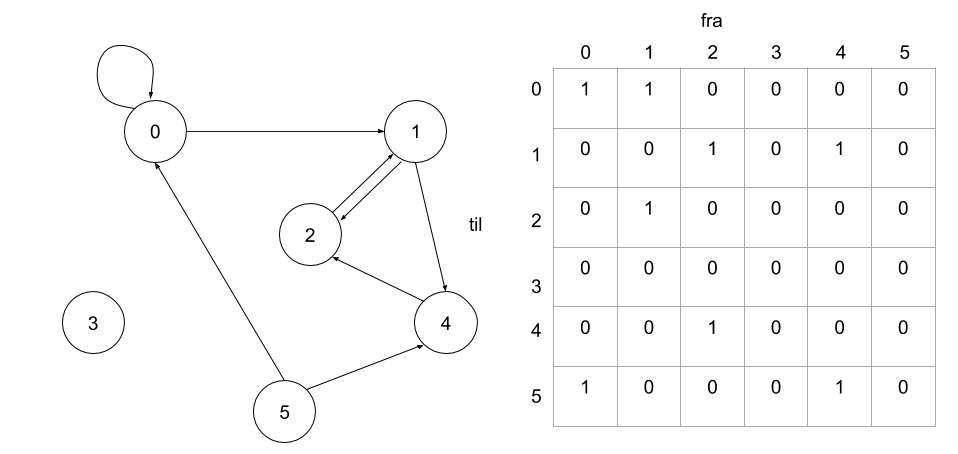
\includegraphics[scale=0.5]{images/implementasjon}
\centering %centering the image
\caption{Implementasjon}
\label{fig:implementasjon}
\end{figure}

\noindent Det finnes flere måter å implementere grafen på; for eksempel kan den representeres som en array av lenkede lister, hvor listen på posisjon \textit{i} forteller hvilke noder som er naboene til node \textit{i}.

\subsection{Representasjon}
\subsubsection{Nabolister}
\subsubsection{Nabomatriser}
\subsection{Traversering}
Her skal vi gjennom to måter å gå systematisk gjennom er graf på. Disse metodene er det veldig vitkig å kunne og forstå.

\subsubsection{DFS: Dybde-først-søk}
Prinsippet er at grafen skal utforskes i dybden. Det betyr at den neste kanten du skal utforske, går fra den noden du sist oppdaget. Dersom denne noden ikke har noen kanter som går til noder du ikke har oppdaget før, går du tilbake til forrige node og gjør det samme der, osv. Kort fortalt går du utover i grafen så langt du kommer før du trekker deg tilbake og går framover igjen så snart du får muligheten til det.
\\\\
Dette prinsippet kan illustreres ed hjelp av en stakk (LIFO). Den noden som ligger på toppen er den neste som skal utforskes. Hvis denne har en kant til en annen node som vi ikke har truffer på før, legges denne nye noden øverst. Hvis den noden som ligger på toppen ikke har noen kanter til en uutforsket node, tas noden ut av stakken og legges i en liste over ferdighbehandlede noder. Ofte er det nok å bare holde rede på om hver node er truffet på eller ikke, men i noen sammenhenger ønsker man å ha en trefarging av nodene: uoppdagede noder er hvite, noder som er oppdaget og fortsatt ligger i stakken er grå, og ferdigbehandlede noder er svarte. Se kapittel 22.3 i Cormen.
\\\\
Legg merke til at dersom det går flere kanter ut fra den noden du skal undersøke til andre uoppdagede noder, spiller det i prinsippet ingen rolle hvilken du velger. Forskjellige valg vil gi forskjellige resultater, men alle vil være gyldige. Når duskal implementere DFS, er det imidlertid greit å bestemme seg for en eller annen regel, for eksempel at naboene skal behandles i alfabetisk rekkefølge, eller i den rekkefølgen de er oppgitt i nabolisten. Merk at hvis noden øverst på stacken, la oss si node \textit{X}, har flere naboer, så skal \textit{ikke} alle slenges inn i stakken på en gang; først skal en av dem, f.eks. node \textit{Y}, legges inn, og så jobber man videre med den. Ikke før node Y er ferdigbehandlet og fjernet fra stacken (og node \textit{X} således dukker opp på toppen igjen) skal man gå videre med neste nabo (hvis denne naboen fremdeles er ubesøkt – det kan jo hende at søket fra node \textit{Y} fant frem hit).
\\\\
Når stacken er tom er du i utgangspunktet ferdig, men der er ikke sikkert ar du nådde ut til hele grafen fra den noden du startet på, for det er ikke alltid det er forbindelse mellom alle nodene i en graf. Dersom du er interessert i å utforske \textit{hele} grafen med DFS må du, hver gang stacken er tom, sjekke om alle nodene er blitt besøkt. Dersom det er flere uoppdagede igjen, dytter du en av dem inn i stacken og starter et nytt DFS derfra. Dette gjentar du til alle nodene er oppdaget.

\begin{boxed}
Vi oppretter stakken "oppdaget", hvor vi legger nodene etterhvert som vi oppdager dem, og listen "ferdig", hvor vi legger de ferdig utforskede nodene.\newline\newline
Vi begynner på A og traverserer grafen etter prinsippene over. Følg med på hvordan vi beveger oss i grafen.

\begin{figure}[H]
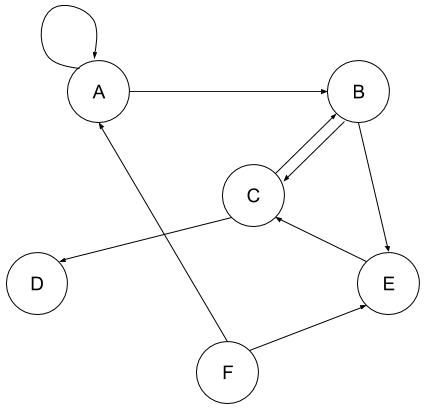
\includegraphics[scale=0.5]{images/DFS}
\centering %centering the image
\caption{Traversering av DFS}
\label{fig:DFS}
\end{figure}

1. oppdaget: A; ferdig: - (A har seg selv som nabo, men A er jo oppdaget, så vi tar B i stedet)\\\\
2. oppdaget: A, B; ferdig: - (B har to naboer, C og E, og vi velger å fortsette med C – men det hadde også vært tillatt å fortsette med E)\\\\
3. oppdaget: A, B, C; ferdig: - (C har B som nabo, men B er oppdaget, så vi tar D i stedet)\\\\
4. oppdaget: A, B, C, D; ferdig: - (D har ingen naboer, så vi er ferdig med D og kan fjerne den fra stacken)\\\\
5. oppdaget: A, B, C; ferdig: D (vi er nå tilbake på C, som ikke har flere ubesøkte naboer, så vi er ferdige med den også)\\\\
6. oppdaget: A, B; ferdig: D, C (B har E som ubesøkt nabo)\\\\
7. oppdaget: A, B, E; ferdig: D, C (E har ingen ubesøkte naboer)\\\\
8. oppdaget: A, B; ferdig: D, C, E (osv.)\\\\
9. oppdaget: A; ferdig: D, C, E, B\\\\
10. oppdaget: -; ferdig: D, C, E, B, A (stakken er tom, så nå går vi gjennom alle nodene og ser etter ubesøkte noder – det viser seg at F er ubesøkt, så vi legger inn den)\\\\
11. oppdaget: F; ferdig: D, C, E, B, A (F har ingen ubesøkte naboer)\\\\
12. oppdaget: -; ferdig: D, C, E, B, A, F (stakken er tom og det er ingen ubesøkte noder igjen; vi er ferdige)
\end{boxed}

\begin{lstlisting}
    function DFS(G,v)	//v er startnode
	    initialiser en tom stack, S
    	for each vertex u in G do
    		set visited[u] $\rightarrow$ false
    	end for
    	S.push(v)
    	while S.notEmpty() do
    		u = S.pop()
    		for all w adjacent to u do
    			if not visited[w] then
    				visited[w] $\rightarrow$ true
    				S.push(w)
    			end if
    		end for
    	end while
    end function
\end{lstlisting}

\subsubsection{BFS: Bredde-først-søk}
Prinsippet er at grafen skal utforskes i bredden. Det betyr at du utforsker alle kantene ut i fra den noden du står i før du beveger deg til neste node. 
\\\\
Dette prinsippet kan illustreres ved hjelp av en kø (FIFO). Den noden som ligger først i køen, la oss kalle den \textit{X}, er den vi skal utforske naboene til. De ubesøkte nodene som \textit{X} har kanter til legges bakerst i køen (rekkefølgen spiller i prinsippet ikke noen rolle her). Deretter fjernes \textit{X} fra køen og legges i en liste med ferdigbehandlede noder.
\\\\
Også her er det mulig at alle nodene ikke er forbundet, men når man bruker BFS, er man som regel kun interessert i nodene som kan nås fra den opprinnelige startnoden. Derfor gir man seg med en gang køen er blitt tom, uten å sjekke om det finnes uoppdagede noder.
\\\\
BFS egner seg godt til å finne ut hvor mange kanter som er nødvendig å bruke for å komme seg fra startnoden til de andre nodene. Grunnen til dette er at det første vi gjør, er å se på alle naboene til startnoden – disse ligger jo 1 kant unna. Deretter vil hver av disse nodene plukkes ut av køen, og alle de ubesøkte naboene deres må nødvendigvis ligge 2 kanter unna startnoden osv. Når vi tar ut en node fra køen kan vi dermed markere alle de ubesøkte naboene dens med en avstand på 1 mer enn nodens egen avstand. Startnoden har naturlig nok avstand 0 til seg selv.

\begin{boxed}
Vi oppretter køen "oppdaget", hvor vi legger nodene etterhvert som vi oppdager dem, og listen "ferdig" hvor vi legger de ferdigbehandlede nodene.

\begin{figure}[H]
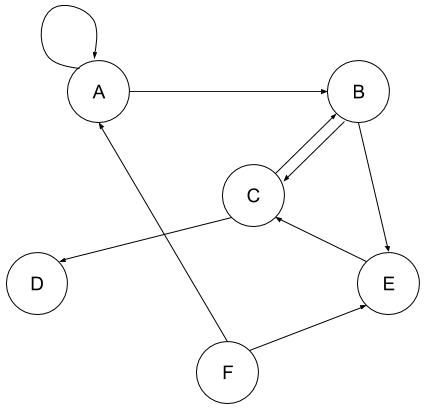
\includegraphics[scale=0.5]{images/DFS}
\centering %centering the image
\caption{Traversering av BFS}
\label{fig:BFS}
\end{figure}
1. oppdaget: A(0); ferdig: - (A sine naboer er A og B, men A er jo allerede oppdaget, så kun B vil legges inn, og avstanden vil bli 1)\\\\
2. oppdaget: B(1); ferdig: A(0) (B sine to naboer er C og E vil legges inn med avstand 2)\\\\
3. oppdaget: C(2); ferdig: A(0), B(1)\\\\
4. oppdaget: E(2), D(3); ferdig: A(0), B(1), C(2) (E har ingen ubesøkte naboer)\\\\
5. oppdaget: D(3); ferdig: A(0), B(1), C(2), E(2)\\\\
6. oppdaget: -; ferdig: A(0), B(1), C(2), E(2), D(3) (Køen er nå tom, og vi er ferdige – F ble ikke besøkt fordi den ikke kunne nås fra A)\\\\
Legg merke til hvordan nodene kommer ut av køen i stigende rekkefølge med hensyn på avstand fra startnoden.
\end{boxed}

\noindent BFS implementeres med en kø. BFS utforsker grafen i bredden. Man starter på foreldrenoden og legger inn alle dens barn i køen. Når alle naboer til node $x$ er oppdaget, fjernes den fra køen og man tar den neste noden i køen og legger alle dens barn inn i køen. Når køen er tom, sjekker man ikke videre om det er ubesøkte noder.

\begin{lstlisting}
    function BFS(G,v) // v er startnode
	    lag en kø Q
    	legg v inn i Q
    	while Q.notEmpty() do
    		v = Q.dequeue()
    		for each edge e adjacent to v do
    			if e not marked then
    				mark w
    				Q.enqueue(e)
    			end if
    		end for
    	end while
    end function

\end{lstlisting}

\subsection{Korteste vei}
Denne typen problemer er ekstremt nyttig i mange sammenhenger. Hvis man skal kjøre bil fra et sted til et annet, vil man gjerne kjøre den korteste veien for å spare bensin og tid. I dette tilfellet holder det å se på veilengden som en kostnad for hver kant. I dette tilfellet blir kostnaden alltid positiv, men det trenger den ikke bli i andre eksempler. Hvis man skal dra rundt og selge ting og er ute etter å se på hvor mye man tjener på forskjellige ruter, kan det hende man vet at det på enkelte strekninger vil bli tap. Men det er fortsatt mulig å finne ut hvilken vei det lønner seg å ta for å tjene mest mulig penger.

\subsubsection{SLOW-ALL-PAIRS-SHORTEST-PATHS}
Tillater ikke negative sykler.

\subsection{Én til alle}
Her vi vil konsentrere oss om de problemene som har ett startpunkt, og som går til alle tenkelige sluttpunkt i den mengden man ser på. Anta at vi er fire studenter som deler kjøkken på Nedre Singsakerslette, og alle har sin egen bil og skal hjem til jul. Førstemann bor i Drøbak, den andre på Kolbotn, nummer tre på Tretten, og fjerdemann i Malvik. Da holder det at man kjører en algoritme for korteste vei, én-til-alle-problem (her kan man også benytte seg av det gunstige faktum at alle kostnader er positive, noe som dere etterhvert vil se gir enklere og raskere algoritme). Med et kart over alle byer og veier i Norge er det bare å bruke Trondheim som startpunkt og kjøre en algoritme for å finne de korteste veiene fra Trondheim til alle de andre byene, og så sjekke rutene man fikk til Drøbak, Kolbotn, Tretten og Malvik. Dermed kan alle ta hver sin bil (ikke så veldig sosialt eller økonomisk, men eksempelets intensjon helliger midlet) og kjøre korteste vei til sin hjemby. 
\\\\
Et viktig prinsipp i alle korteste-vei-problemene, er det som kalles \textbf{relaxation}. Dette er ikke noe mer skummelt enn at man sjekker en eller annen kant fra en node \textit{u} til en annen node \textit{v}, og skulle denne kanten tilby en kortere vei til \textit{v} enn den veien vi eventuelt hadde fra før, oppdaterer man node \textit{v} med informasjon om at den korteste veien nå kommer fra node \textit{u}. Skulle den veien man prøver være lenger, oppdaterer man ikke.

\begin{figure}[H]
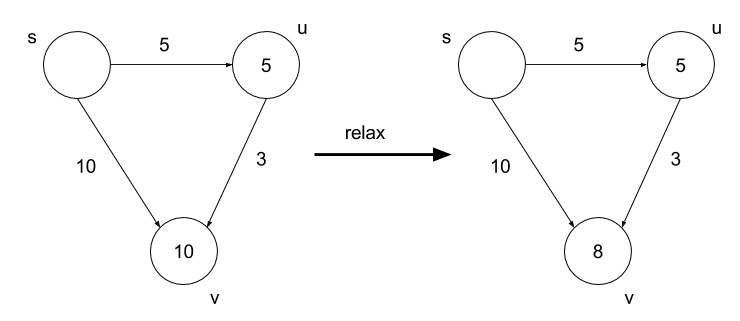
\includegraphics[scale=0.5]{images/relaxation}
\centering %centering the image
\caption{Relaxation. Tallet i noden angir funnet avstand fra kilden.}
\label{fig:relaxation}
\end{figure}

\noindent En viktig ting å ha i mente, er at korteste vei \textbf{ikke kan ha sykler}. Har man en \textbf{positiv sykel}, så vil man ved å fjerne denne sykelen fortsatt ha en vei mellom sine to noder som også blir kortere enn om man brukte sykelen. Har man en sykel med verdi 0, så blir denne helt uniteressant, og man kan like godt droppe den. Hvis det eksisterer en \textbf{negativ sykel}, så vil man kunne gå rundt denne negative sykelen så mange ganger man vil og få stadig kortere vei. Dermed vil det ikke kunne være en bestemt korteste vei, da man alltid kan ta en ny runde i den negative syklen og få en enda kortere vei. Negative sykler ødelegger faktisk hele problemstillingen, og ingen av algoritmene våre vil klare å finne noe godt svar dersom grafen inneholder en negativ sykel som kan nås fra startnoden. Merk dog at en graf kan inneholde negative kanter uten å ha negative sykler.

\subsubsection{BELLMAN-FORD}
Denne algoritmen tar for seg de problem hvor kostnadene på kantene til grafen kan være negative. Dermed blir den ganske generell. Hvis det eksisterer negative sykler, returnerer Bellman-Ford "FALSE". Men om slike negative sykler ikke forekommer (vel og merke holder det at de ikke kan nås fra utgangspunktet vårt), så returnerer algoritmen beste vei.
\\\\
Algorimen fungerer som følger (se også s. 588 i Cormen):
\begin{enumerate}
    \item La antall noder i grafen være \textit{|V|}. Følgende gjøres \textit{|V| - 1} ganger: Gå gjennom alle kantene og kjør \textit{relax} på hver av dem. Når man er ferdig med dette, vil man faktisk ha funnet den korteste veien (vel og merke om man ikke har en negativ sykel). Studér kommende eksempel, og prøv å forstå hvorfor det må bli slik – ta gjerne \textit{path-relaxation property} fra side 587 i Cormen til hjelp (den sier at hvis kantene på den korteste veien mellom to  noder blir "relaxed" i riktig rekkefølge, selv hvis det foregår mange andre relaxations imellom, vil man få en riktig verdi for korteste avstand). Alle veier mellom nodene vil være utprøvd, og den korteste veien blir funnet takket være path relaxation property.
    \item Deretter gjelder det å finne ut om vi faktisk har en negativ sykel. Dette gjør man ved å sjekke samtlige kanter i grafen. La oss si at vi har en kant fra node \textit{u} til node \textit{v}, kann denne kanten (\textit{u,v}). Hvis summen av kostnaden fra startnoden til node \textit{u} og kostnaden til (\textit{u,v}) blir mindre enn verdien vi fant for kostnaden fra startnoden til \textit{v}, vil dette bety at man har en negativ sykel. Dette bevises i Cormen på side 590.
\end{enumerate}

\noindent Hvis man kaller antallet noder for \textit{|V|} og antallet kanter for \textit{|E|}, blir kjøretiden til Bellman-Ford-algoritmen ganske enkelt $O(|V||E|)$. Dette ser man lett, da man går gjennom alle nodene en gang for hver gang man tar for seg en node vil man måtte sjekke et antall kanter som er proposjonalt med antallet kanter som eksisterer. For å sjekke negative sykler tar det bare $\theta(|E|)$ i tid, så denne vil ikke påvirke den asymptotiske kjøretiden fra første del av algoritmen.

\begin{figure}[H]
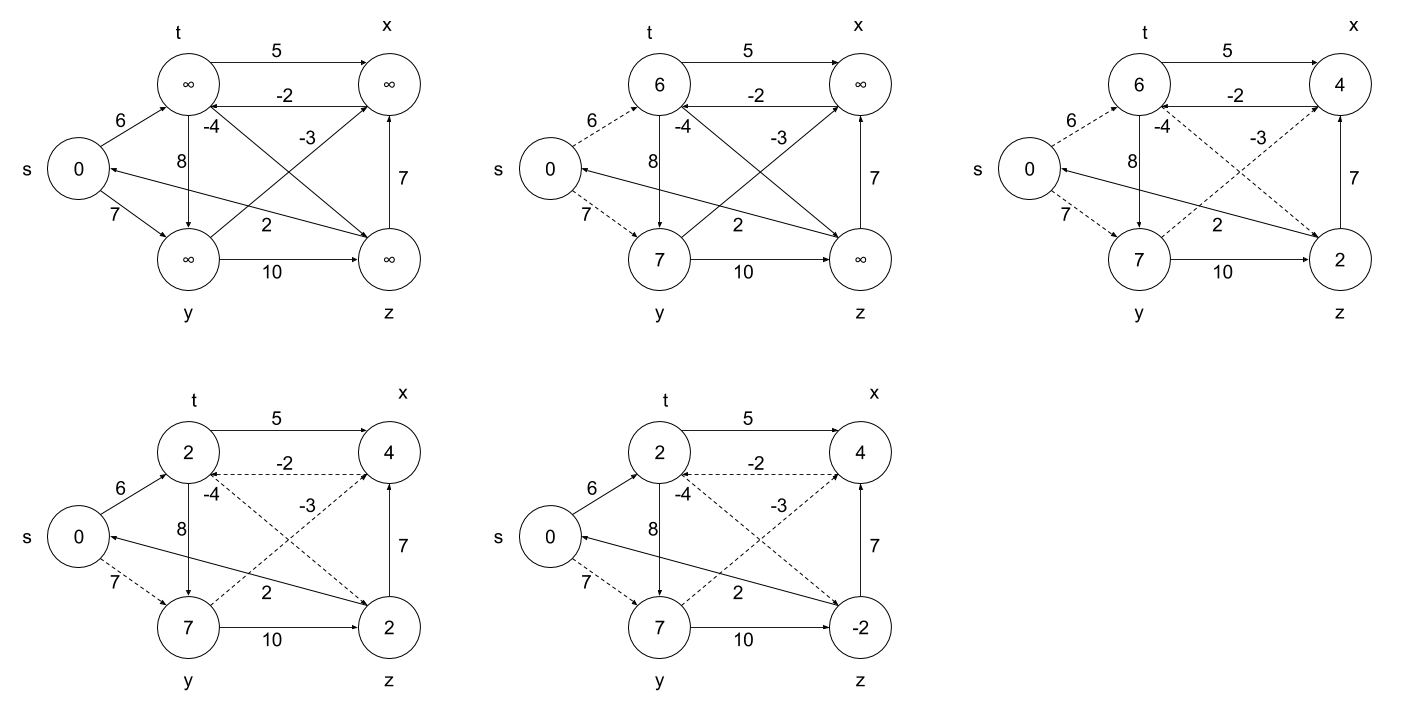
\includegraphics[scale=0.3]{images/bellman-ford}
\centering %centering the image
\caption{Bellman-Ford}
\label{fig:bellman-ford}
\end{figure}

\subsubsection{DIJKSTRAS ALGORITME}
Kravet for å bruke Dijkstras algoritme er at alle kantene har positive verdier (eventuelt også verdien 0). Da kan man bruke en smartere algoritme enn Bellmann-Ford. Dijkstrra er faktisk en \textbf{grådighetsalgoritme}. Pseudokode står på side 595 i Cormen.
\\\\
Dijkstra er en korteste vei, en-til-alle-algoritme. Tillater ikke negative kanter. Den velger noder en etter en fra hvor nærme de er startnoden. 
\\\\
Det faktum at grågighetsprinsippet fungerer her, gjør at man kan kjøre gjennom en algoritme som ikke tester alt det som Bellmann-Ford måtte ha testet. Hvorfor grådighet vil fungere, er ikke så vanskelig å se for seg. Hvis du bruker 10 liter bensin bort til Ola og 15 liter til Mogens, vil det aldri i verden kunne være lønnsomt å dra via Mogens til Ola hvis vi ser på bensinforbruket. For vi må nødvendigvis svi av noe bensin mellom Ola og Mogens, så uansett hva vi forbruker mellom disse to fyrene vil det fra et bensin-perspektiv være ulønnsomt å dra via Mogens (ja, det finnes selvsagt argumenter for å besøke Mogens. Det kan jo være direkte hyggelig, og dessuten gir han deg kanskje bensin gratis. Men i dette tilfellet vil denne bensinen Mogens gir deg regnes som et negativt forbruk, og vi kan ikke bruke Dijkstra).
\\\\
Kort fortalt plukker Dijkstra ut nodene en etter en ut fra hvor nær de er startnoden hvis vi følger korteste vei. Den første noden som plukkes ut er startnoden (husk at dette er en én-til-alle-algoritme). Deretter kjøres relaxation til alle andre noder for å finne neste node som skal plukkes ut tas ikke med i neste runde med relaxation. Dette gjentas til vi har funnet korteste vei til alle nodene. 

\begin{boxed}
En gjeng syklister er samlet på startstreken (startnoden) til et sykkelritt. Alle er like spreke og sykler nøyaktig like fort hele tiden. Vi lar kostnaden mellom to noder være tiden det tar for en syklist å sykle fra den ene til den andre. Målet i et tradisjonelt sykkelritt er selvsagt å komme først i mål, men her er det snakk om å finne korteste vei til alle nodene.\newline\newline
Det er mange veilvalg underveis, men vi antar at det er så mange syklister at det alltid er minst en til hvert veivalg. Slik vil den eller de syklisten(e) som besøker en node først, ha funnet den korteste veien til denne noden og tiden han/de brukte illustrerer kostnaden til denne veien.
\newline\newline
Det er akkurat slik Dijkstra finner de korteste veiene; så fort en syklist når fram til en hittil ubesøkt node, legges den til i mengden med noder vi har funnet kortest vei til.
\end{boxed}

\begin{figure}[H]
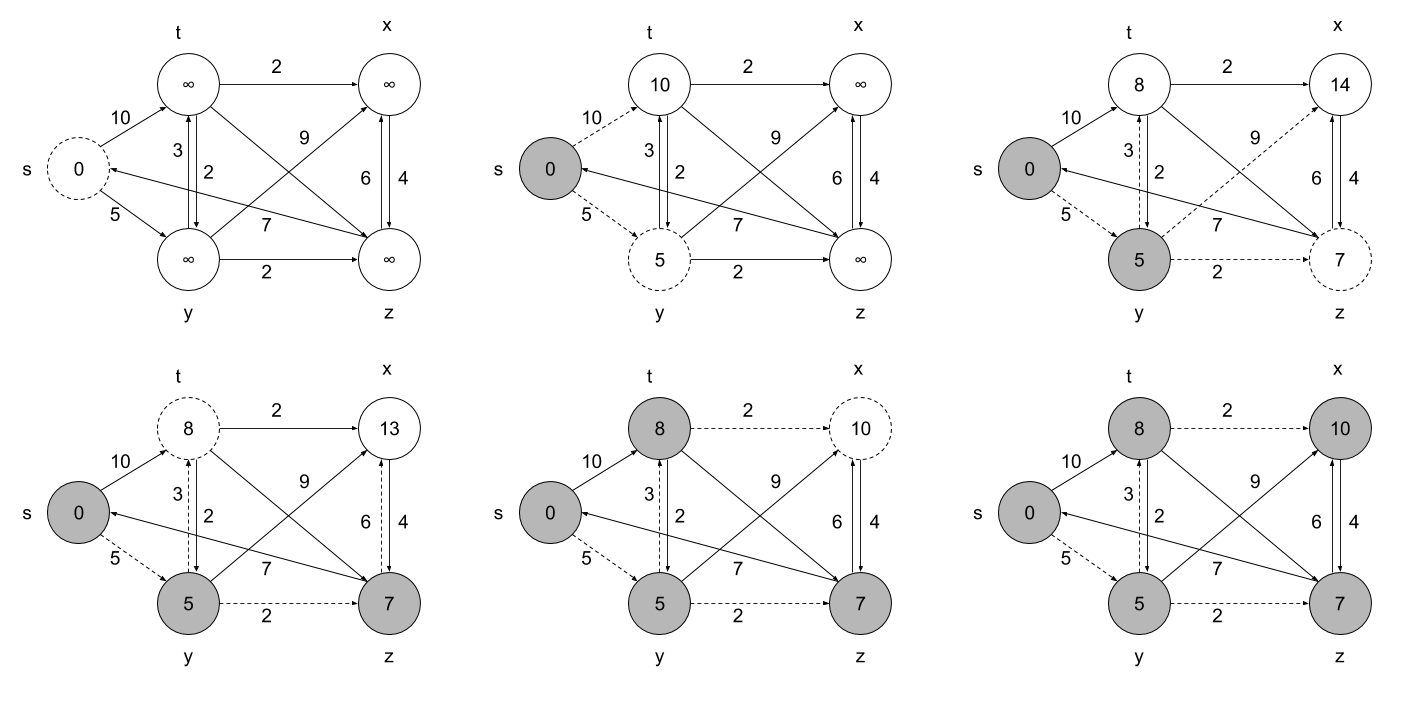
\includegraphics[scale=0.3]{images/dijstra}
\centering %centering the image
\caption{Dijkstra}
\label{fig:dijkstra}
\end{figure}

\noindent Det kan vises at kjøretiden til Dijkstra er $O(|V|^2)$ i de fleste tilfeller, men den kan gjøres bedre om man har god kunnskap om grafen man ser på. Merk at $O(|V|^2)$ er bedre enn $O(|V||E|)$, fordi antallet kanter $|E|$ minst må være $|V| - 1$ mens den øvre grensen faktisk kan være asymptotisk med $|V|^2$.

\begin{lstlisting}
    function DIJKSTRA(G,w,s)
	    INITIALIZE-SINGLE-SOURCE(G,s)
    	S = Ø
    	Q = G.V
    	while Q $\neq$ Ø do
    		u = EXTRACT-MIN(Q)
    		S = S $\cup$ {u}
    		for each vertex v $\in$ G.Adj[u] do
    			RELAX(u,v,w)
    		end for
    	end while
    end function
\end{lstlisting}

\noindent Hvis man har en DAG, vil det ikke oppstå noen vanskeligheter selv om man har negative kostnader på kantene, for i en DAG vil det ikke eksistere noen sykler i alle tilfeller. Trikset for å finne korteste vei er i første rekke å gjøre en topologisk sortering av DAGen. Slik oppnår vi en lineær ordning av nodene. Deretter trenger vi bare besøke nodene en gang i den topologisk sorterte rekkefølgen og kjøre en relaxation for hver gang til de noder som ligger foran. 
\\\\
Kjøretiden vil avhenge av den topologiske sorteringen, og en slik sortering har kjøretid $\theta(|V|+|E|)$. Ingen andre ledd i algoritmen for korteste vei i en DAG vil bli større enn den topologiske sorteringen, så kjøretiden blir $\theta(|V|+|E|)$.

\subsubsection{DAG shortest path}
DAG-Shortest-Path er en korteste vei, en-til-alle algoritme. Tillater ikke negative kanter, og kan selvfølgelig ikke ha sykler, da det er en DAG. Gjør topologisk sortering av DAGen og besøker hver node en gang for å kjøre RELAX på nodene foran.

\begin{lstlisting}
    function DAG-SHORTEST-PATH(G,w,s)
    	TOPOLOGICAL-SORT(G)
    	INITIALIZE-SINGLE-SOURCE(G,s)
    	for each vertex u, taken in topologically sorted order do
    		for each vertex v ∈ G.Adj[u] do
    			RELAX(u,v,w)
    		end for
    	end for
    end function
\end{lstlisting}

\subsubsection{RELAX}

\subsection{Alle til alle}
En soleklar måte å takle dette problemet på, er rett og slett å bruke en god algortime for et én-til-alle-problem, og så bruke denne på samtlige noder som startnoder. Dette er ikke så dumt som det kan høres ut som. Hvis alle kostnadene er ikke-negative, fungerer det meget bra å bruke Dijkstra. Kjøretiden her vil bli $O(|V|^3)$, som man ser ved å multiplisere kjøretiden til en gjennomgang av Dijkstra med antallet noder $|V|$. Hvis vi har negative kostnader og kjører samme trikset med Bellman-Ford, blir kjøretiden $O(|V|^2 |E|)$, som ikke er så veldig bra fordi $|E|$ er av størrelsesorden $|V|^2$. Nå skal det sies at med meget smarte fremgangsmåter her, vil disse kjøretidene kunne senkes betraktelig. Men vi bruker heller en algoritme som tar for seg problemet med alle-til-alle uten å skulle gå omveien om mange gjennomkjøringer av en én-til-alle-algoritme.

\subsubsection{FLOYD-WARSHALL}
Ved å benytte oss av prinsippet om \textbf{dynamisk programmering} skal vi her vise hvordan Floyd-Warshall-algoritmen fungerer. Antar at det ikke finnes negative sykler i input.
\\\\
Pseudokoden for Floyd-Warshall er relativt grei. Man lager en nabomatrise til nodene, men gjør litt om på den. Hvis det går en vei fra en node til en annen, setter vi verdien til å være kostnaden på kanten mellom dem. Går det ikke en direkte kant mellom de to nodene, settes kostnaden til å være uendelig ($\infty$). Deretter velger man seg en node, kall noden \textit{a}, som man har lov til å gå innom. Så tester man veien mellom to og to noder, kall dem \textit{u} og \textit{v}. Hvis det koster mindre å gå via \textit{a}, så legger man inn denne veien til å være den korteste. Nå har vi en oversikt over de korteste veiene som kun består av enkeltkanter eller som bruker node \textit{a} (og ingen andre). Så kan vi gå videre og tillate en annen node, \textit{b}, og sjekke om vi kan få kortere veier ved å ta den i bruk osv. Etter å ha gått gjennom alle nodene på denne måten vil vi til slutt ha en oversikt over de korteste veiene uten noen begrensninger på hvilke noder som kan brukes. Det er heller ikke så veldig vanskelig å lage enda en nabomatrise som holder styr på hvilke noder man skal gå innom for å oppnå denne ultimate veien. Det er ikke så rent ulogisk at dette vil fungere, men det gjelder å få et godt grep om hva som skjer.

\begin{figure}[H]
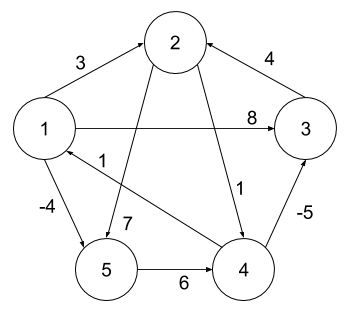
\includegraphics[scale=0.5]{images/floyd-warshall}
\centering %centering the image
\caption{Floyd-Warshall. Tallene i noden betyr her nummeret på noden, ikke avstand.}
\label{fig:floyd-warshall}
\end{figure}

\noindent Figuren viser grafen til problemet vårt. Om vi bruker algoritmen på siden 630 i Cormen, vil matrisene under utregning bli slik du ser under her. Merk at indeksen i hver matrise betyr hvilken node vi har gått innom. Den første, med indeks 0, er startmatrisen. 
\\\\
\noindent Kjøretiden til Floyd-Warshall er ganske enkelt $O(|V|^3)$. Det er $|V|$ noder man skal innom, og for hver gang kan man variere startnoden med $|V| - 1$ muligheter og sluttnoden med $|V| - 2$ muligheter. Om man ser på pseudokoden i Cormen, så ser man at den består av tre greie for-løkker. Nå skal det sies at også Dijkstra på alle nodene gir $O|V|^3$, men operasjonen per ledd i Floyd-Warshall er så mye mindre at denne stort sett vil lønne seg selv hvis alle kantene er positive. Dersom det er relativt få kanter i forhold til noder vil derimot Dijkstra med heap (som kjører på $O(|E| lg |V|)$ for hver av de $|V|$ nodene) lønne seg.

\subsubsection{TRANSITIVE-CLOSURE}

\subsubsection{FASTER-ALL-PAIRS-SHORTEST-PATHS}
Har en kjøretid på $\theta(n^3 lg n)$. Tillater ikke negative sykler.

\subsection{Maksimal flyt}
I stedet for å la kostnaden til kanten mellom to noder representere avstand eller pris, som i Floyd-Warshall, så er det i noen situasjoner gunstig å operere med en kapasitet og en flyt mellom nodene. Denne flyten kan være meget generell, så maks-flyt-problemer spenner over et stort område. I et maks-flyt-problem ønsker vi å finne den største flyten fra en gitt kilde til et gitt sluk uten å overskride noen kapasitetskrav.

\subsubsection{Flytnettverk}
Et flytnettverk $G = (V,E)$ (hvor V står for nodene og E for kantene) er en rettet graf hvor hver kant (\textit{u,v}) har en ikke-negativ kapasitet $c(u,v) \geq 0$. Eksisterer det ingen kant mellom to noder, setter vi kapasiteten til å være null. To av nodene er av spesiell betydning. Det er kilden \textit{s}, som er den eneste noden som kan produsere flyt, og sluket \textit{t}, som er den eneste noden som kan ta imot flyt uten å sende den videre. Vi kan nå definere flyt på følgende måte:
\begin{center}
En flyt i G er en funksjon: $f: V * V \rightarrow$  ${\Bbb R}$
\end{center}

\noindent slik at følgende tre krav er oppfylt:
\begin{itemize}
    \item \textbf{Kapasitet:} For alle \textit{u, v} $\in V$ så krever vi $f (u,v) \leq c (u,v)$. Flyten må altså ikke overstige kapasiteten.
    \item \textbf{Symmetri:} For alle $u,v \in V$ så krever vi $f (u,v) = -f(v,u)$. Positiv flyt én vei tilsvarer altså en like stor, negativ flyt motsatt vei (akkurat som når man regner på strøm i elektriske kretser).
    \item \textbf{Bevaring av flyt:} For alle $v \in V - \{s,t\}$ (altså for alle noder \textit{v} unntatt kilden og sluket) krever vi at flyten inn må være like stor som flyten ut, dvs. at det ikke "renner over" i noen noder og at ingen noder kan produsere flyt selv. Det kan formuleres som at summen av flyten inn i \textit{v} må være null:
    \begin{center}
    $\sum\limits_{u \in V} f(u,v) = 0$ 
    \end{center}
\end{itemize}

\noindent Det første kravet sier at vi alltid må respektere kapasiteten. Det andre kravet er egentlig bare en formalitet som gjør det mulig å regne med negativ flyt, som generaliserer teorien en hel del. Hvis jeg sender hundre kroner til din konto, vil de gå en positiv flyt av penger fra meg til deg, mens det går en negativ flyt fra deg til meg. Bevaringsloven til sist sier bare at flyt ikke uten videre kan forsvinne eller oppstå. Dette kan sammenlignes med diverse bevaringslover fra fysikken, som f.eks. energibevaring.
\\\\
Vi sier at $|f|$ er flyten fra kilden til sluket, og dens verdi er rett og slett summen av flyten til alle veiene ut fra kilden, som igjen er det samme som summen av flyten inn i sluket. Mer presist:
\begin{center}
    $|f| = \sum\limits_{u \in V} f(s,v)$ 
    \end{center}
    
\noindent Legg spesielt merke til siste krav, som gir at total flyt i en node må være null. Det som kommer inn blir sendt ut igjen med samme rate, det er ingenting som hoper seg opp. Dette kan sammenlignes med Kirchoffs lover for elektrisk strøm. Ellers er den totale positive flyten definert til å være summen av de positive flytene inn i en node, eller:
\begin{center}
    $\sum\limits_{u \in V, f(u,v)>0} f(u,v) = 0$ 
    \end{center}
    
\noindent Hvis vi har flere kilder og sluk, er det et godt triks å legge til en superkilde og et supersluk, slik at vi oversetter problemet til det vi er vant til. Dette gjøres ved å opprette en ny node med kanter til alle kildene. Sett kapasiteten på disse kantene til uendelig (med mindre du ønsker å sette noen spesielle begrensninger på flyten). Tilsvarende skal alle slukene ha en kant til supersluket. I alle videre utregninger skal du tenke på superkilden/-sluket som eneste kilde/sluk.

\begin{figure}[H]
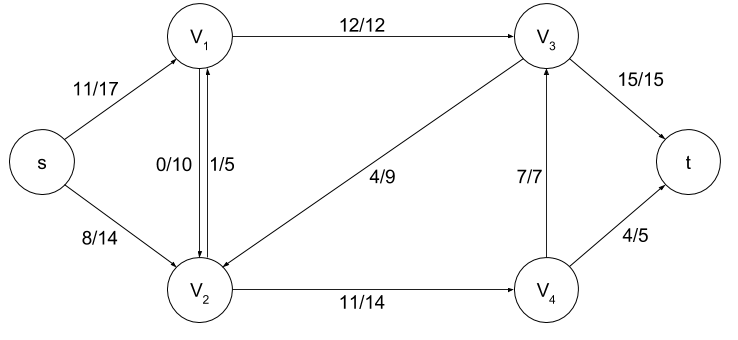
\includegraphics[scale=0.6]{images/flytnettverk}
\centering %centering the image
\caption{Flytnettverk}
\label{fig:flytnettverk}
\end{figure}

\subsubsection{FORD-FULKERSONS METODE}
Ideen her er å finne en eller annen flytforøkende vei \textit{p} og øke flyten \textit{f} på hver kant til \textit{p} med residualkapasiteten. Fremgangsmåten er så enkel som at man rett og slett finner en flytforøkende vei, og når man har gjort det setter man på all den flyten som veien kan tåle. Deretter leter man etter en ny flytforøkende vei, og gjør det samme. Når man oppdager at det ikke er mer flytforøkende veier, har man oppnådd maksimal flyt. Dette kalles for Ford-Dulkerson-metoden. Grunnen til at det ikke kalles for en algoritme er at det ikke er spesifisert hvordan man skal finne den flytforøkende veien. Måten man gjør dette på kan få drastisk innvirkning på kjøretiden.
\\\\
Det som kan være urovekkende, er altså hvordan man skal sjekke om det eksisterer en flytforøkende vei. Et av de bedre triksene, er å bruke et bredde-først-søk. Hvis man kombinerer Ford-Fulkersons-metoden med BFD kalles det for Edmonds-Karp-algoritme.

\begin{boxed}
Vi starter med et nettverk uten noe flyt. Det som er stiplet er en flytforøkende vei. Gangen blir som vist i Figur \ref{fig:ford-fulkerson}.

\begin{figure}[H]
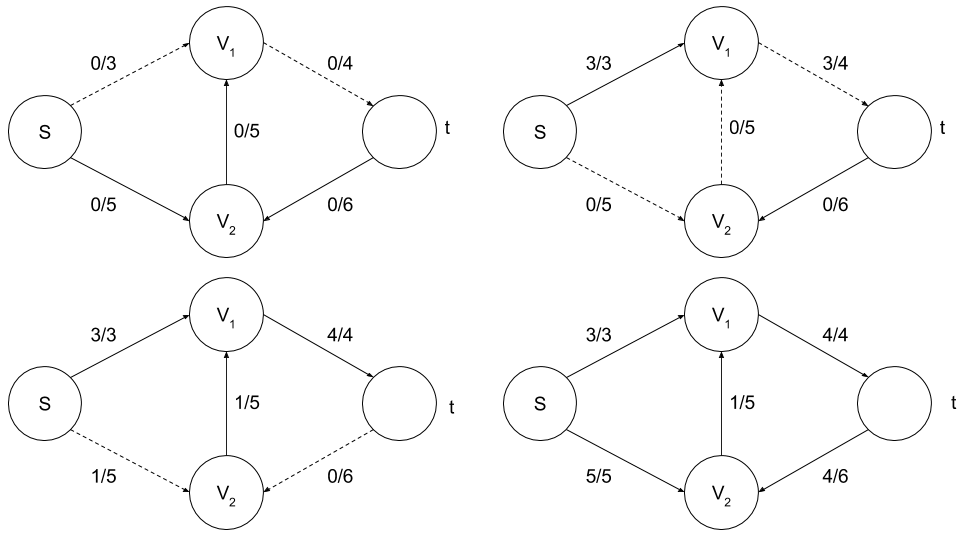
\includegraphics[scale=0.45]{images/ford-fulkerson}
\centering %centering the image
\caption{Ford-Fulkerson}
\label{fig:ford-fulkerson}
\end{figure}
\end{boxed}

\noindent Hvis kapasitetene er heltall, vil man ha at kjøretiden til Ford-Fulkerson er $O(E|f^*|$, hvor $f^*|$ er den maksimale flyten, og $E$ som vanlig er antallet kanter. Dette ser man greit ved at man for hvert søk risikerer å måtte gå gjennom alle kantene, og man vil sende minst én enhet av flyten hver gang. Legg merke til at Ford-Fulkerson ikke hadde fungert dersom vi hadde hatt irrasjonale kapasiteter.  
\\\\
Ford-Fulkerson-metoden er en god algoritme som finner maksimal flyt i et flytnettverk. Hver iterasjon forsøker å finne en flytforøkende sti, og setter på all den flyten som er mulig. Deretter leter den etter en ny flytforøkende sti, og gjentar prosessen. Når det ikke er flere flytforøkende stier har man oppnådd maksimal flyt. Den benytter seg av DFS for å finne flytforøkende sti. Det er altså tre essensielle ideer; residualnettverk, flytforøkende vei, og snitt.\\

\subsection{Residualnettverk}
Som uttrykket kanskje tilsier ("residual" betyr "rest"), for et flytnettverk med en gitt flyt, består residual-nettverket av de kantene som tillater mer flyt. Gitt et flytnettverk \textit{G} og en flyt $f$, da skriver vi $G_f$ for residualnettverket.

\begin{boxed}
Vi beskriver ofte flyten og kapasiteten ved å skrive en brøk med flyt-verdien øverst og kapasitetsverdien nederst. Man får residual-nettverket ved å ta de opprinnelige kapasiteter og trekke fra den flyten som går i hver kant. Med flyten fra Figur \ref{fig:flytnettverk} får vi residualnettverket til å bli som vist i Figur \ref{fig:residualnettverk}.

\begin{figure}[H]
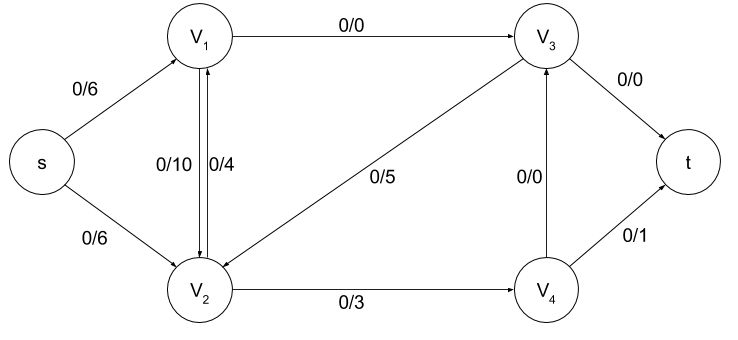
\includegraphics[scale=0.6]{images/residualnettverk}
\centering %centering the image
\caption{Residualnettverk}
\label{fig:residualnettverk}
\end{figure}
\end{boxed}

\subsubsection{Flytforøkende sti}
En flytforøkende vei er rett og slett en enkel vei fra kilden $s$ til sluket $t$ i residualnettverket $G_f$. I Figur \ref{fig:flytforokendevei} er den stiplede veien en flytforøkende vei. Vi ser at vi kan sende en enhet i den flytforøkende vieen.

\begin{figure}[H]
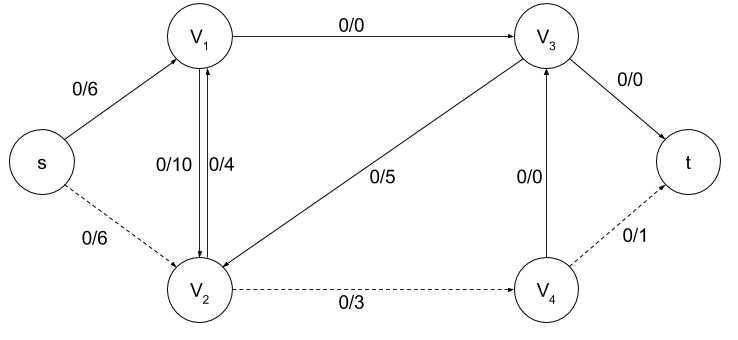
\includegraphics[scale=0.6]{images/flytforokendevei}
\centering %centering the image
\caption{Flytforøkende vei}
\label{fig:flytforokendevei}
\end{figure}

\subsubsection{Snitt}
Vi definerer et snitt som følger:
\begin{center}
    Et snitt $(S,T)$ til et flytnettverk $G = (V,E)$ er en partisjon av nodene $V$ i $S$ og $T = V - S$ slik at kilden $s$ ligger i $S$ og sluket $t$ ligger i $T$.
\end{center}
\noindent Med andre ord er snittet en inndeling av alle nodene i to deler hvor kilden og sluket er i hver sin del. Vi snakker om nettoflyt og kapasitet over et snitt, hvor det førstnevnte er all flyten gjennom snittet fra kilden til sluket minus kapasitet fra sluk til kilde. Et minimalt snitt er et snitt hvis kapasitet er den minste oppnåelige.

\begin{figure}[H]
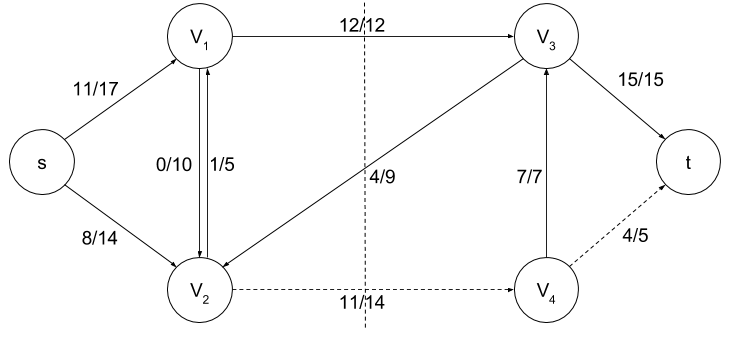
\includegraphics[scale=0.6]{images/snitt}
\centering %centering the image
\caption{Snitt}
\label{fig:snitt}
\end{figure}

\noindent Det vises i Cormen at flyten gjennom et snitt $(S,t)$ rett og slett er $|f|$. Om man skjønner hva dette står for, er resultatet temmelig trivielt. Det sier bare at den flyten som sendes fra kilden og går inn i sluket, i sin helhet må krysse snittet. Ved å se på figuren over, ser man at dette er tilfellet. Tenker man litt etter, så vil man innse at dette enkle resultatet medfører det faktum at flyten $f$ i et flytnettverk $G$ har en øvre begrensning ved kapasiteten til ethvert snitt. Av dette følger et meget viktig teorem:
\begin{center}
    Hvis $f$ er en flyt i et flytnettverk $G = (V,E)$ med kilde $s$ og sluk $t$, så er de følgende utsagnene ekvivalente (det vil si at hvis vi vet en av dem, vet vi de andre også):
    \begin{enumerate}
         \item $f$ er en maksimal flyt i $G$
        \item Residualnettverket $G_f$ har ingen flytforøkende vei
        \item Verdien på flyten fra kilde til sluk, $|f|$ må være lik kapasiteten til et eller annet snitt.
    \end{enumerate}
\end{center}

\noindent For å si det enkelt, det å finne det minimale snittet er det samme som å finne den maksimale flyten. Ved å tenke seg om, er dette ganske greit. Når vi har maksimal flyt, så vil det bli "kork" der hvor kapasiteten er minst, og ingenting mer kan slippe gjennom denne flaskehalsen. Det hjelper for eksempel ikke uten videre å legge trefelts motorvei fra Oslo mot svinesund når veien ut fra Oslo består av én fil. For å finne et minimalt snitt (det kan finnes flere) når man først har funnet maksimal flyt kan man gjøre et bredde-først-søk gjennom residualgrafen fra (super)kilden. De nodene man når frem til er på kildens side.

\subsubsection{EDMONDS-KARP}
Endret en bokstav på Ford-Fulkerson-metoden. De benytter seg av BFS. Edmonds-Karp bruker Ford-Fulkerson og BFS til å finne flytforøkende stier.\\

\subsection{Topologisk sortering}
La oss si at nodene representerer oppgaver som skal gjøres. Noen oppgaver må gjøres før andre. For eksempel må du lage middagen før du kan spise den. Andre kan gjøres i valgfri rekkefølge. Dette kan illustreres med en rettet graf.
\\\\
Topologisk sortering går ut på å finne en mulig rekkefølge oppgavene kan gjøres og tar utgangspunkt i en DAG. Det er opplagt at topologisk sortering bare har mening når vi har å gjøre med en rettet graf, og den kan ikke inneholde sykler. Dersom vi har sykler eksisterer ingen gyldig løsning.

\begin{boxed}
\begin{figure}[H]
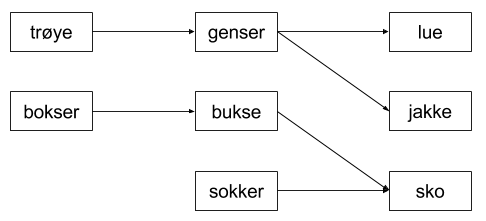
\includegraphics[scale=0.7]{images/topologisk}
\centering %centering the image
\caption{Topologisk sortering}
\label{fig:topologisk}
\end{figure}

Et klassisk eksempel er rekkefølgen du kan kle på deg. I grafen har vi tatt men noen klesplagg, og pilene viser rekkefølgen de må tas på. Det kan selvsagt diskuteres om du må vente med å ta på deg luen til du har tatt på deg genseren, men av erfaring blir det gjerne ekstraarbeid dersom du forsøker annen rekkefølge.
\end{boxed}

\subsubsection{Algoritme}
Topologisk sortering er veldig enkelt når du har forstått DFS. Du kjører rett og slett bare et DFS og lager en liste med oppgavene i den rekkefølgen de fjernes fra stakken. Deretter reverserer du listen, og du vil da ha en gyldig rekkefølge å utføre oppgavene i. Grunnen til at dette virker er at når en node \textit{X} fjernes fra stakken, vet du at du har utforsket alle pilene ut fra \textit{X}, og dermed har vi allerede utforsket de nodene som avhenger av \textit{X} og lagt dem til i listen. Vi kan dermed legge til \textit{X}, og når listen reverseres, vil \textit{X} stå foran alle nodene som avhenger av den.

\begin{boxed}
Vi må begynne traverseringen i en node som ikke har noen piler inn mot seg. Minst én slik node vil finnes, da grafen ikke har noen sykler. Vi kan altså begynne med enten trøye, bokser eller sokker.\newline\newline
Vi velger å begynne med "sokker" (nok en gang er det tillatt å velge fritt blant de aktuelle alternativene). Disse legges øverst i stakken. Vi har bare en vei å gå videre, nemlig til "sko". Ingen piler peker fra "sko", så vi kan være sikre på å ikke besøke noden i grafen igjen, og legger derfor "sko" først i listen \textit{besøktForSisteGang}. Vi går så tilbake til "sokker", og oppdager at heller ikke denne noden kjenner noen noder vi ikke har besøkt enda. "Sokker" legges så til i listen \textit{besøktForSisteGang}. Nå er listen \textit{oppdaget} tom igjen, og vi må søke for å se om det er flere noder i grafen. Det er det, men vi må passe på å velge en som ikke har noen kanter inn mot seg. Vi velger "bokser". Det fører til at "bukse" og "bokser" blir puttet inn i \textit{besøktForSisteGang} i den rekkefølgen. Vi finner så "trøye", går videre til "genser", og velger tilfeldigvis "lue" før "jakke". "Lue" kjenner ingen flere og blir lagt til i \textit{besøktForSisteGang}. Vi går tilbake til "genser", som også kjenner "jakke". "Jakke", "genser" og "trøye" blir lagt til i listen i denne rekkefølgen.
\\\\
Etter at traverseringen er ferdig, ser listen \textit{besøktForSisteGang} slik ut: "sko", "sokker", "bukse", "bokser", "lue", "jakke", "genser", "trøye". Vips, så har du en mulig rekkefølge å ta på deg klærne i, nemlig først trøye, så genser, jakke, lue, bokser, bukser, sokker og til slutt sko. Dette er kanskje ikke den rekkefølgen du velger til vanlig, men det er ingen praktisk grunn til at du ikke skulle kunne kle på deg i denne rekkefølgen, i alle fall ikke ut i fra den miniverdenen grafen gir oss. Du kan selvsagt argumentere for at du ikke vil ta på deg jakke og lue før frokost, men vil gjerne ha på deg bokser først. Dette er imidlertid umulig å se ut ifra grafen, men hvis dette var veldig viktig for deg kunne du ha lagt inn piler fra "bokser" til "jakke" og "lue". Da ville den endelige rekkefølgen ha blitt annerledes.
\end{boxed}